\subsection{Relation}
\label{sec:Suggestion:Relation}

The \textsf{Relation} part provides traceability links between \textsf{MM}
and all the corresponding \textsf{changed} and \textsf{impacted} elements.
One \textsf{MM} element change
may impact several elements in the same \viewtype, but may also potentially
impact several \viewtypes. We only require so-called \emph{links}; however richer
data structures for traceability may be used \cite{Batot-Cabot-Gerard:2021}.

The way these traceability links are computed are left as implementation
details, and may happen in two ways: \emph{statically}, when \viewtypes are defined,
by filtering links relevant to changes from a pool of general links available;
or \emph{dynamically} after a change session. This may happen \emph{on-the-fly},
whenever an \textsf{MM} element is evolved; or \emph{offline},
after a complete evolution session has terminated --- either based on diffing 
\cite{Kehrer-Kelter-Taentzer:2011}, or using operation-based approaches \cite{J:Lippe-Oosterom:1992}.

\begin{figure}[t]
    \centering
    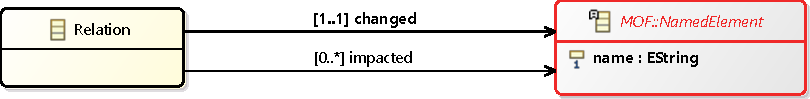
\includegraphics[width=\columnwidth]{Relation.pdf}
    \caption{\textsf{Relation}s between \textsf{MM} elements and \textsf{VT} elements.}
    \label{fig:Relation}
\end{figure}

In the \textsf{FSM} example associated to the initial \textsf{VT\_FSM} of \cref{fig:VT:VMM},
we would have, among others, the following relations (with \textsf{Link}s denoted 
as e.g.~$\mathsf{<} \mathsf{changed} ; \mathsf{impacted} \mathsf{>}$):
\begin{itemize}
	\item Since computing the \textsf{name}s in \textsf{VT\_FSM} requires access
	to $\mathsf{Named \squaredots name}$, the following \textsf{Link}s would be
	created: 
	$\mathsf{<} \mathsf{Named \squaredots name} ; \mathsf{VT\_FSM \squaredots name} \mathsf{>}$;
	$\mathsf{<} \mathsf{Named \squaredots name} ; \mathsf{State \squaredots name} \mathsf{>}$;
	$\mathsf{<} \mathsf{Named \squaredots name} ; \mathsf{Transition \squaredots name} \mathsf{>}$.

	\item Creating an instance of \textsf{State} requires to take into account
	the value of $\mathsf{State \squaredots kind}$, which would produce the following
	\textsf{Link}s: 
	$\mathsf{<} \mathsf{State \squaredots kind} ; \mathsf{State} \mathsf{>}$;
	$\mathsf{<} \mathsf{State \squaredots kind} ; \mathsf{Initial} \mathsf{>}$;
	$\mathsf{<} \mathsf{State \squaredots kind} ; \mathsf{Regular} \mathsf{>}$.
	Depending on the precision of the traceability analysis, the following may
	eventually be produced as well: 
	$\mathsf{<} \mathsf{Kind \squaredots REGULAR} ; \mathsf{Regular} \mathsf{>}$ and
	$\mathsf{<} \mathsf{Kind \squaredots INITIAL} ; \mathsf{Initial} \mathsf{>}$.
	%\LC{Again, for FINAL too?}\MA{The \textsf{Link}s are established on the initial version, \emph{\textbf{before} the evolution step. 
	%The next bullet (``After Step 2''!!!) explicitly says what you want to put here, which is a wrong place to do so.}}
	


	\item After Step 2, some \textsf{Link}s between the newly added attributes
	in $\mathsf{FSM \squaredots Transition}$ and the corresponding attributes in 
	$\mathsf{VT\_FSM \squaredots Transition}$ may be added as well. New 
	\textsf{Link}s taking into account the newly added literal in \textsf{Kind}
	would be added, similarly to the previous point.
\end{itemize}